\documentclass[journal,twoside,web]{ieeecolor}
\usepackage{tmi}
\usepackage{cite}
\usepackage{mathtools,amssymb,amsfonts}
\usepackage{algorithmic}
\usepackage{graphicx}
\usepackage{textcomp}
\usepackage{hyperref}
\usepackage{empheq} % for algorithms
\usepackage{mdframed} % for algorithms

\newtheorem{theorem}{Theorem}
\newtheorem{lemma}[theorem]{Lemma}
\newtheorem{proposition}[theorem]{Proposition}
\newtheorem{corollary}[theorem]{Corollary}

\newcommand{\R}{\mathbb{R}}

\DeclareMathOperator*{\argmin}{\text{\rm{argmin}}}

\def\BibTeX{{\rm B\kern-.05em{\sc i\kern-.025em b}\kern-.08em
    T\kern-.1667em\lower.7ex\hbox{E}\kern-.125emX}}
\markboth{\journalname, VOL. XX, NO. XX, XXXX 2020}
{Author \MakeLowercase{\textit{et al.}}: Preparation of Papers for IEEE TRANSACTIONS ON MEDICAL IMAGING}

\begin{document}
\title{Title}
\author{First A. Author, \IEEEmembership{Fellow, IEEE}, Second B. Author,and Third C. Author, Jr., \IEEEmembership{Member, IEEE}
\thanks{This paragraph of the first footnote will contain the date on which
you submitted your paper for review. It will also contain support information,
including sponsor and financial support acknowledgment. For example, 
``This work was supported in part by the U.S. Department of Commerce under Grant BS123456.'' }
\thanks{The next few paragraphs should contain the authors' current affiliations,
including current address and e-mail. For example, F. A. Author is with the
National Institute of Standards and Technology, Boulder, CO 80305 USA (e-mail:author@boulder.nist.gov). }
\thanks{S. B. Author, Jr., was with Rice University, Houston, TX 77005 USA.
He is now with the Department of Physics, Colorado State University,
Fort Collins, CO 80523 USA (e-mail: author@lamar.colostate.edu).}
\thanks{T. C. Author is with the Electrical Engineering Department,
University of Colorado, Boulder, CO 80309 USA, on leave from the National
Research Institute for Metals, Tsukuba, Japan (e-mail: author@nrim.go.jp).}}

\maketitle

\begin{abstract}
Diffusion MRI (dMRI) is a powerful imaging technique for probing tissue microstructure by capturing the displacement of water molecules. Reconstructing meaningful representations from undersampled dMRI data, however, remains a challenging task—especially when aiming beyond standard low-dimensional models such as DTI or HARDI. In this work, we propose a novel reconstruction framework that directly targets the full Ensemble Average Propagator (EAP), a probability density function (PDF) describing local diffusion. Our method operates in joint
(k,q)-space and leverages an Optimal Transport-inspired Total Variation (TV) regularization to recover high-resolution spatial and diffusion information from sparse measurements.

At the core of our approach is a regularizer that extends classical TV to PDF-valued functions using a generalized 1-Wasserstein distance, adapted to handle non-normalized data. This formulation promotes spatial coherence while respecting the geometry of displacement distributions. Additionally, we include a complementary voxel-wise smoothing term in displacement space to enhance robustness. We implement our variational model with a primal-dual algorithm and validate it on synthetic and semi-realistic datasets featuring complex fiber configurations. The results show that our method correctly reconstructs crossing patterns of heavily undersampled and noisy inputs, offering a promising alternative to high-resolution dMRI.
\end{abstract}

\begin{IEEEkeywords}
Enter about five key words or phrases in alphabetical order, separated by commas.
\end{IEEEkeywords}

\section{Introduction}
\label{sec:introduction}
\IEEEPARstart{D}{iffusion} Magnetic Resonance Imaging (Diffusion-MRI or dMRI) is a powerful non-invasive imaging technique that is able to capture the microscopic diffusion of water molecules in biological tissues, thus providing information on microstructures, particularly in neural, muscular, and fibrous tissues, where diffusion is directionally constrained by cellular architecture.

In classical MRI, spatial information is encoded in $k-$space, the Fourier domain of the spatial image. Each point in k-space corresponds to a frequency. In dMRI, on the other hand, an additional encoding is introduced by sensitizing the MRI signal to diffusion using additional gradient pulses. The resulting signal becomes dependent not only on the spatial frequency (k) but also on the diffusion dimension (q), which encodes the direction and strength of diffusion-sensitizing gradients. Sampling in q-space allows for the reconstruction of the diffusion Probability Density Functions (PDF), which describe the full displacement distribution for each spatial coordinate.

In principle, Diffusion Spectrum Imaging (DSI) requires the acquisition of the full $(k,q)$ spectrum and can be prohibitively time-consuming in practical applications, leading to unbearably long scan times \cite{wedeen2005mapping,wedeen2008diffusion}. Solutions to this problem usually require the reconstruction of a smaller object, and the employment of Compressed Sensing (CS) approaches \cite{menzel2011accelerated,bilgic2012accelerated}. Popular techniques that combine both are, for example, Diffusion Tensor Imaging (DTI) \cite{basser1994estimation} and High Angular Resolution Diffusion Imaging (HARDI) \cite{tuch2002high,frank2002characterization,alexander2002detection}; both are instances of so-called Q-Ball imaging routines \cite{tuch2004q,descoteaux2007regularized}, and as such do not allow for a full spectrum reconstruction, neglecting information on the intensity of the displacement, and the former is even intrinsically unable to detect fiber crossings.

To address the challenge posed by DSI, recent work has focused on undersampling strategies in both k-space and q-space, giving rise to the concept of joint (k,q)-space sampling. In this high-dimensional space, neither spatial nor angular frequencies are fully sampled. The task of reconstruction from undersampled (k,q)-space data is a highly ill-posed inverse problem and demands the use of advanced tools to recover both high-quality images and diffusion information. One common approach for solving inverse problems as well as in this particular instance, is the use of a Tikhonov-type regularization, such as the Total Variation (TV) functional and its variants, which have become popular in the Inverse Problems community thanks to their favorable properties and relative ease of use.

Classical TV has been introduced for the restoration of noisy images, given its ability to promote sparsity in the gradient, thus favoring the recovery of piecewise constant solutions. In the same spirit, we employ a generalization of TV that is tailored to the DSI case, i.e. which is meant to be applied to PDF-valued functions (formalized here as measures), based on Optimal Transport theory, offering new ways to incorporate geometric priors and structural correlations into the reconstruction.

\subsection{Brief overview of Diffusion MRI}
The object we aim to reconstruct is the Ensemble Average Propagator (EAP) $\bar{P}(x,r)$, representing the probability that a water molecule at position $x \in \R^3$ (voxel space) displaces by a vector $r \in \R^3$. Thus, the physical process underlying Diffusion-MRI involves the encoding of both spatial and diffusion information through magnetic field gradients. When diffusion-sensitizing gradients are applied, the resulting MRI signal becomes sensitive to the displacement of water molecules. This interaction can be mathematically modeled as a {Fourier-type encoding} of the displacement process. The quantity that is actually measured by the scanner is the signal \( E(k,q) \), which is related to the EAP via the six-dimensional Fourier transform
\begin{align}
    E(k,q) =
    \int_{\R^3}\int_{\R^3} \rho(x) \, \bar{P}(x,r) \, e^{-2\pi i(k \cdot x + q \cdot r)} dx dr,
\end{align}
where $k$ is the spatial frequency vector associated with the MRI spatial gradients, $r$ is the displacement variable in real space, $q$ is the diffusion gradient vector in q-space and $\rho(x)$ is the proton (or spin) density at position $x$.

The signal $E$, which is the only one that can be physically acquired, is subject to noise and, given its high-dimensional nature and the underlying acquisition technology, undersampling strategies become mandatory. The undersampling process can be modeled as a linear operator $\mathcal{U}$, and defining the \emph{weighted displacement distribution} as
\[
P(x,r) := \rho(x) \, \bar{P}(x,r),
\]
the signal can be rewritten more compactly as
\begin{align}\label{eq:EAP Fourier}
    E = \mathcal{U(F}(P)),
\end{align}
where \( \mathcal{F} \) denotes the six-dimensional Fourier transform in the \((x, r)\) variables. In the following, we will still refer to $P$ as the Ensemble Average Operator.

Common and established approaches to the dMRI problem prescribe shell acquisitions, where diffusion gradients are sampled on one or more spheres in q-space, corresponding to fixed b-values. These acquisition schemes are the basis of Q-ball imaging techniques, including DTI and HARDI, which only recover partial information about the EAP.

In contrast, our framework operates directly in the full six-dimensional $(x,r)$ space and is designed to jointly regularize across both spatial and displacement domains. This enables the incorporation of structural priors that couple anatomical continuity with the geometry of molecular displacement, opening new possibilities for recovering richer diffusion representations from heavily undersampled $(k,q)$ data.

\subsection{Related work and contributions}
\textit{This approach is quite new, so there are few directly related works \cite{VogtLellmann1}, .\\
TV-regularization applied to MRI and in particular Diffusion-MRI.
Experimental application of the theory to anatomically-respondent models; propose another unbalanced version of Optimal Transport distance; introduction of an extra regularizing smoothing term; analysis of the involved parameters; review of the literature and introduction to non-specialist public. Use of a novel fiber-tracking method?}

\section{Method}

\subsection{Theoretical background}
\subsubsection{Total Variation} Given an open, bounded domain $\Omega \subset \R^d$ and a smooth function $f:\Omega \to \R$, the Total Variation of $f$ is defined as
\begin{align}
    \mathrm{TV}(f) = \int_\Omega \| \nabla f(x) \| dx
\end{align}
where $\| \cdot \|$ is a norm on $\R^d$, typically the Euclidean or the $1$-norm; the former choice produces what is called \textit{isotropic} TV, which carries better denoising properties, while the latter gives the \textit{anisotropic} TV, which can be handled more easily in numerical algorithms for separability reasons. In short, the TV provides a measure of how ``jagged" the graph of $f$ is and, if used as an additive regularizer, it encourages piecewise constant solutions and is therefore well suited for mitigating noisy measurements. If $\Omega$ is a (for simplicity two-dimensional) discrete grid, these choices reduce, respectively, to
\begin{subequations}\label{eq:TV standard discrete}
\begin{alignat}{3}
  & \mathrm{TV^{\,i}}(f) \label{eq:TV standard iso} & & = \sum_{(i,j)\in\Omega}\sqrt{(f_{i+1,j}-f_{ij})^2 + (f_{i,j+1}-f_{ij})^2 } \\
  & \mathrm{TV^a}(f) \label{eq:TV standard aniso} & & = \sum_{(i,j)\in\Omega} | f_{i+1,j}-f_{ij} | + | f_{i,j+1}-f_{ij} |
\end{alignat}
\end{subequations}
with zero boundary conditions as later specified in section \ref{sec:Equivalent formulation}.

The TV functional has been used in a variety of fields, from classical image denoising tasks to medical imaging problems, including X-ray Tomography, Functional MRI and PET deconvolution [\textit{add citations}]. Although several generalizations have been proposed (including, e.g., for vector- and matrix-valued functions [add citations]), few constitute a tight match for the Diffusion-MRI problem. This needs indeed to encompass the more general case of maps valued in a space of functions, as the EAP from \eqref{eq:EAP Fourier} can be thought as
\begin{align}
    P : \Omega \to \mathcal{X}
\end{align}
where $\mathcal{X} \subseteq \{ g: \R^3 \to \R\}$. Adopting this point of view, authors in \cite{TVW_Theory} proposed to use a specific metric on the space $\mathcal{X}$, derived from Optimal Transport theory [Villani]. The idea is that, under certain assumptions, one could directly mimic \eqref{eq:TV standard discrete}. Suppose, for instance, that a meaningful distance $d$ is available on $\mathcal{X}$; then one may define, in the anisotropic case,
\begin{align} \label{eq:TV^a_d}
    \mathrm{TV}_d(P) = \sum_{(i,j)\in\Omega} d(P_{i+1,j},P_{ij}) + d(P_{i,j+1},P_{ij}) \, .
\end{align}
This is the approach followed, for example, in \cite{LeveragingEAP}, where $d(P_1,P_2) = \| P_2 - P_1 \|_1$, amounting to employ an $L^1$-TV regularization (jointly with a term promoting sparsity in a suitable surfacelet transform). In the present work, $d$ will be derived from the so-called 1-\textit{Wasserstein} distance $W_1$.
\subsubsection{Optimal Transport}
Optimal Transport studies distances between probability measures defined as the minimization of some transport cost. For example, a classical choice is the 1-Wasserstein distance: for $\bar{P}_1,\bar{P}_2$ probabilities on $Y$
\begin{align} \label{eq:definition of W1}
    W_1(\bar{P}_1,\bar{P}_2) = \min_{\gamma\in\Gamma(\bar{P}_1,\bar{P}_2)} \int_{Y\times Y}|y_1-y_2| d\gamma(y_1,y_2) \, ,
\end{align}
where $|\cdot|$ is the Euclidean norm (or the Frobenius norm for higher-dimensional arrays - we will keep this notation throughout this manuscript) and $\Gamma(\bar{P}_1,\bar{P}_2)$ stands for the set of probabilities on the product space $Y \times Y$ having $\bar{P}_1$ and $\bar{P}_2$ as first and second marginals. This definition may look abstract at first but its interpretation is straightforward: a fixed $\gamma\in\Gamma$ prescribes how $\bar{P}_1$ should be mapped to $\bar{P}_2$, while the integral returns the corresponding transport cost. The minimization requires that the mapping should be as ``frugal" as possible: every mass point in the starting distribution $\bar{P}_1$ should be sent to a ``nearest" point in a way that globally matches $P_2$. Note that $\bar{P}_1$ and $\bar{P}_2$ are not required to be probability measures strictly, but they must have the same total mass — otherwise, they cannot be marginals of a common coupling $\gamma$. Also, the 1-Wasserstein distance scales linearly with mass, a property that is important in unbalanced settings [\textit{cite Lellmann, cite La Torre}].

An alternative and often more tractable expression of the 1-Wasserstein distance is given by its dual formulation, commonly referred to as the \textit{Kantorovich–Rubinstein} formulation:
\begin{align} \label{eq:KR}
    W_1(P_1,P_2) = \max_{\mathrm{Lip(f)}\le 1} \int_Y f(y) (P_2(y)-P_1(y)) dy
\end{align}
where $\mathrm{Lip}(f)$ denotes the Lipschitz constant of a function $f:Y \to \R$. 
This formulation is convenient and will serve as the basis for our method. Note, first, that the constraint in \eqref{eq:KR} involves objects of the same dimensionality as the probability measures, as opposed to the quadratic size of transport plans $\gamma$
in \eqref{eq:definition of W1}. Second, the constraint can be expressed locally via the gradient of $f$,
\begin{align} \label{eq:constraint Lipschitz local}
    \sup_{y_1 \neq y_2} \frac{|f(y_2) - f(y_1)|}{|y_2 - y_1|} = \mathrm{Lip}(f) \le \alpha \iff \| \nabla f \|_\infty \le \alpha \, ,
\end{align}
which constitutes a considerable numerical advantage.

From this notion of Optimal Transport distance, other variations or extensions of the $W_1$ have been proposed, which can measure the discrepancy between measures with different masses. In \cite{TVW_Theory}, for example, the authors suggest the use of an unbalanced version $\widetilde{W}_1$, which is essentially a mixture of the $W_1$ and of the $L^1$-norm.
% \begin{align*}
%     \widetilde{W}_1(P_1,P_2) = \min_{ \substack{ \|Q_1\|_1 = \|Q_2\|_1 } } W_1(Q_1,Q_2) + \|P_1-Q_1\|_1 + \|P_2-Q_2\|_1
% \end{align*}
Here, we propose the following: for $P_1,P_2$ measures on $Y$
\begin{align} \label{eq:W1 hat}
    \hat{W}_1^{\alpha_1,\alpha_2}(P_1,P_2) = \alpha_1 W_1(J(P_1),J(P_2)) + \alpha_2 \big| I(P_1) - I(P_2) \big|
\end{align}
where $\alpha_1,\alpha_2>0$, $I$ returns the sum of the entries of its argument (which is the total mass in the case of a positive measure) and $J$ is a linear operator, that makes sure the resulting masses are equal, i.e. $ I(J(P_1)) = I(J(P_2)) $.
Specifically, $I(P_1) = \mathbf{1} \cdot P_1 = \sum_i (P_1)_i$, $\mathbf{1}$ being the vector of ones, and $J$ projects onto the space of zero-mean functions by subtracting the constant component: $J(P_1):= \mathrm{id} - \tfrac{1}{N} I^*I$ if $P_1$ has size $N$.
The intuition behind definition \eqref{eq:W1 hat} is simple: given one way $J$ to normalize the distributions to the same mass, this unbalanced distance corresponds to the $W_1$ between the normalized measures, penalized by the difference in mass. Two advantages of such a definition are that it properly generalizes the Optimal Transport distance $W_1$ (i.e. $W_1({P}_1,{P}_2) = \hat{W}_1({P}_1,{P}_2)$ whenever $P_1$ and $P_2$ are probability measures - which is not always the case for $\widetilde{W}_1$), and that it makes the variational problem slightly lighter by reducing the size of one dual variable.

We will therefore employ $\mathrm{TV}_{\hat{W}_1}^{\alpha_1,\alpha_2}$, or $\mathrm{TV}_{\hat{W}_1 }$ for short, as outlined in \eqref{eq:TV^a_d}, with $d=\hat{W}_1^{\alpha_1,\alpha_2}$.

\subsection{Variational problem}
To carry out the discussion around the relevant variational problem, we fix discrete, 2-dimensional grids $\Omega$ and $Y$
\begin{align*}
    \Omega &= \{ 1, \dots, m_1 \} \times \{ 1, \dots, m_2 \},\\
    Y &= \{ 1, \dots, n_1 \} \times \{ 1, \dots, n_2 \}
\end{align*}
representing the spacial and displacement domains, respectively, so that the EAP
\[ P:\Omega \times Y \to \R \]
can be written as a vector $ P \in \R^{m_1 \times m_2 \times n_1 \times n_2} $. The choice of 2-D grids is purely for notational convenience, and nothing changes for higher dimensional models (for example, in 2D echo planar imaging protocols, where each slice is acquired independently and the data is reconstructed slice-by-slice, $\Omega$ is 2-dimensional and $Y$ is 3-dimensional, while in the full acquisition case, both domains are 3-dimensional).

Our problem will take the standard form of a data-fitting term and a regularization term. For the data fitting, we will choose a simple squared $L^2$-norm of the residual. The main regularization term will be the Optimal Transport-based Total Variation $\mathrm{TV}_{\hat{W}_1}$, discussed above.

In addition to the regularization $\mathrm{TV}_{\hat{W}_1}$, which acts on the spatial domain, we propose the implementation of another TV-type regularizer, encouraging smoothness voxelwise, i.e. in the displacement domain. This is favorable since prior knowledge on the smoothness of the displacements is understood, and this modification can still be embedded into the framework provided by \cite{TVW_Theory}. The smoothing regularizers we put forward for an EAP $P:\Omega \times Y \to \R$ are, with boundary conditions as will be specified in section \ref{sec:Equivalent formulation},
\begin{subequations}\label{eq:TV voxelwise}
\begin{alignat}{3}
  \label{subeq:Dirichlet_Y}
  & \mathrm{Dir}_Y(P) & &
  = \frac{1}{2} \sum_{\substack{ (i,j)\in\Omega \\ (k,l)\in Y }} ( P_{ij,k+1,l}-P_{ijkl} )^2 + ( P_{ij,k,l+1}-P_{ijkl} )^2 \\
  \label{subeq:TV_Y}
  & \mathrm{TV}_Y(P) & & = \sum_{\substack{ (i,j)\in\Omega \\ (k,l)\in Y }} | P_{ij,k+1,l}-P_{ijkl} | + | P_{ij,k,l+1}-P_{ijkl} |
\end{alignat}
\end{subequations}
i.e. a Dirichlet energy (promoting voxelwise smooth solutions) and Total Variation (promoting voxelwise piecewise constant solutions), respectively. As we will further notice in section \ref{sec:Equivalent formulation}, both instances \eqref{subeq:Dirichlet_Y} and \eqref{subeq:TV_Y} can be written as
\begin{align} \label{eq:voxelwise regularization compact}
    \frac{1}{p} \| \nabla_YP\|_p^p
\end{align}
with $p=2$ and $p=1$, respectively.

Putting everything together, the variational problem for reconstructing the EAP from an undersampled measured signal $E$ reads:
\begin{align} \label{eq:variational problem}
    \min_{P:\Omega\times Y \to \R}
    \tfrac{1}{2}| \mathcal{K}(P)-E|^2 + \mathrm{TV}_{\hat{W}_1}^{\alpha_1,\alpha_2}(P) + \tfrac{\beta}{p} \| \nabla_Y P\|_p^p
\end{align}
where $\alpha_1,\alpha_2,\beta > 0$ are the regularization parameters, $\mathcal{K} = \mathcal{UF}$ is an undersampled Fourier transform, $P$ is the EAP variable, $E$ is the undersampled, noisy measured signal and $p\in\{1,2\}$.

\subsection{Equivalent formulation} \label{sec:Equivalent formulation}

To solve \eqref{eq:variational problem}, we recast it in the standard primal–dual form, which is well-suited for first-order optimization methods:
\begin{align} \label{eq:general primal-dual problem}
    \min_x \max_u F(x) - G(u) + \langle Lx , u \rangle
\end{align}
where $F$ and $G$ are proper (i.e. not always equal to $+\infty$), convex, lower semicontinuous functions, $L$ is a linear operator and $\langle \cdot , \cdot \rangle $ is the euclidean product. If $F$ and $G$ are well-behaved (namely, their proximal operator can be easily computed and they satisfy so-called qualification conditions for the min-max problem) several algorithms in the context of Fenchel-Rockaferral duality allow to treat \eqref{eq:general primal-dual problem}, such as the popular primal-dual method by Chambolle and Pock (\textit{cite}), namely the\\

\noindent\textbf{Primal-Dual iteration:}
\begin{equation}
\begin{aligned}
x^{(i+\frac{1}{2})} &= \operatorname{prox}_{\tau F}\big( x^{(i)} - \tau L^* u^{(i)} \big) \\
u^{(i+\frac{1}{2})} &= \operatorname{prox}_{\sigma G}\big( u^{(i)} + \sigma L (2 x^{(i+\frac{1}{2})} - x^{(i)}) \big) \\
x^{(i+1)} &= x^{(i)} + \rho^{(i)} \big( x^{(i+\frac{1}{2})} - x^{(i)} \big) \\
u^{(i+1)} &= u^{(i)} + \rho^{(i)} \big( u^{(i+\frac{1}{2})} - u^{(i)} \big)
\end{aligned}
\label{alg:CP}
\end{equation}
whose implementation will be discussed in the next section. In order do so, we will follow and adapt the track outlined in \cite{TVW_Theory}.

Let us first introduce the notation for the discrete partial differential operators: given a function $P:\Omega \times Y \to \R$, $\nabla_\Omega P$ and $\nabla_Y P$ stand for the finite forward difference gradients in the first and last variables of $P$, respectively:
\begin{align*}
    (\nabla_\Omega P)_{ijkl}
    & = \big(P_{i+1,jkl}-P_{ijkl} \ , \, P_{i,j+1,kl}-P_{ijkl} \big) \\
    (\nabla_Y P)_{ijkl}
    & = \big(P_{ij,k+1,l}-P_{ijkl} \ , \, P_{ijk,l+1}-P_{ijkl} \big)
\end{align*}
with the convention that the outermost differences are zero (i.e. the operators come with homogeneous Neumann boundary conditions, or symmetric padding). This notation will come in handy in more than one instance in the following. As it is common practice, we will also write $\nabla$ for the discrete forward difference gradient on a 2-dimensional grid.

Next, we define the linear operators $\mathbf{I}$ and $\mathbf{J}$, which simply apply $I$ and $J$ entrywise for each $(i,j)\in\Omega$:
\begin{align*}
    (\mathbf{I}P)_{ij} &= I(P_{ij}) \in \R \\
    (\mathbf{J}P)_{ij} &= J(P_{ij}) \in \mathcal{P}(Y) \, .
\end{align*}
In this way, the $\mathrm{TV}_{\hat{W}_1}$ regularizer conveniently splits as
\begin{align} \label{eq:TV unbalanced as sum of TVs}
    \mathrm{TV}_{\hat{W}_1}^{\alpha_1,\alpha_2}(P) = \alpha_1 \mathrm{TV}_{W_1}(\mathbf{J}P) + \alpha_2 \mathrm{TV}(\mathbf{I}P)
\end{align}
Then, by applying the dual formulation \eqref{eq:KR} of $W_1$ together with the observation on the Lipschitz constraint from \eqref{eq:constraint Lipschitz local}, we get
\begin{alignat*}{2}
    \mathrm{TV}_{{W}_1}(P) = & \sum_{ij} &   & \max_{\| \nabla f^1_{ij} \|_\infty \le 1} \langle         JP_{i+1,j} - JP_{ij} , f^1_{ij} \rangle \\
                        &           & + & \max_{\| \nabla f^2_{ij} \|_\infty \le 1} \langle JP_{i,j+1} - JP_{ij} , f^1_{ij} \rangle
\end{alignat*}
that can be written compactly as
\begin{align} \label{eq:TV_W1 temporary}
\mathrm{TV}_{{W}_1}(P) = \max_{\| \nabla_Y f \|_{2,\infty} \le 1} \langle \nabla_\Omega \mathbf{J} P , f \rangle \, ,
\end{align}
where $f:\Omega \times Y \to \R^2$ and the constraint displays the compact notation
\begin{align} \label{eq:norm 2,infty for lipschitz constraint}
    \| \nabla_Y f \|_{2,\infty} = \max_{ \substack{ (i,j) \in \Omega \\ (k,l) \in Y } } \max  \big\{  |(\nabla_Y f^1)_{ijkl}|, |(\nabla_Y f^2)_{ijkl}| \big\} \, ,
\end{align}
which is still in the form of a linear operator composed with a norm, and the compact notation is thus legitimate.

Similarly, the second term in the sum \eqref{eq:TV unbalanced as sum of TVs} can be written as a maximum via the dual norm
\begin{align} \label{eq:TV on masses}
    \mathrm{TV}(\mathbf{I}P) = \| \nabla \mathbf{I}P\|_1 = \max_{ \| g \|_\infty \le 1 } \langle \nabla \mathbf{I} P , g \rangle \, .
\end{align}

Let us now observe that both $\mathrm{Dir}_Y$ and $\mathrm{TV}_Y$ from \eqref{eq:TV voxelwise} depend on $\nabla_Y P$; moreover, the former can be expressed as a sum of pointwise 2-norms squared, and the latter as a full 1-norm, which justifies the notation in \eqref{eq:voxelwise regularization compact}.

Finally, to reach our goal of shaping \eqref{eq:variational problem} into \eqref{eq:general primal-dual problem}, we need a couple of results about convex duality. First, let us introduce two definitions. Given a function $\varphi:\R^n \to (-\infty,+\infty]$, its \textit{convex conjugate} is the function $\varphi^*:\R^n \to (-\infty, + \infty]$ such that
\begin{align*}
    \varphi^*(v) = \sup_{x \in \R^n} \langle v,x \rangle - \varphi(x) \, .
\end{align*}
The Fenchel-Moreau Theorem ensures that if $\varphi$ is proper, convex and lower semicontinuous, then the convex conjugacy is an involution, i.e.
\begin{align*}
    (\varphi^{*})^* = \varphi \, .
\end{align*}
Given a set $C \subseteq \R^n$, the indicator function of $C$ is $\mathcal{I}_C:\R^n \to (-\infty,+\infty]$ such that
\begin{align*}
    \mathcal{I}_C(x) =
    \begin{cases}
        0 & \text{ if } x \in C\\
        +\infty & \text{ otherwise } 
    \end{cases}
\end{align*}
The indicator function is commonly used in Convex Optimization to encode the constraints in the objective function, so that any variational problem can be framed as an  equivalent unconstrained problem, since the arguments that output values at $\infty$ cannot constitute a solution. For example, constraints of the form $\|Ax\|\le 1$, $A$ being a linear operator, can be encoded within the objective function as $\mathcal{I}_B(Ax)$, where $B = \{ x\in \R^n : \|x\| \le 1 \}$ is the closed unit ball. This is also the case for \eqref{eq:TV on masses}), which becomes
\[ \alpha_2 \mathrm{TV({\mathbf{I}P)}} = \max_g \langle \nabla \mathbf{I}P,g \rangle - \mathcal{I}_{B^\infty}(\tfrac{1}{\alpha_2}g) \]
If $C$ is nonempty, closed and convex (as it happens for $B$) its indicator function is proper, convex and lower semicontinuous, so that the Fenchel-Moreau Theorem applies. Moreover, for a closed ball, we have the following result.
\begin{lemma} \label{lemma:conjugate of indicator}
    Let $\| \cdot \|$ be a norm on $\R^n$ and let $\| \cdot\|_*$ be its dual norm, i.e.
    \begin{align*}
        \|y\|_* = \max_{\|x\|\le1} \langle y, x \rangle \, .
    \end{align*}
    If we set $B = \{ x\in \R^n : \|x\| \le 1 \}$ to be the unit ball, then the convex conjugate of the indicator function of $B$ is the dual norm:
    \begin{align*}
        \mathcal{I}_B^* = \| \cdot\|_* \, .
    \end{align*}
\end{lemma}
This means that \eqref{eq:TV_W1 temporary} can be further massaged into
\begin{align*}
    \alpha_1\mathrm{TV}_{W_1}(P) &= \alpha_1\max_f \langle \nabla_\Omega\mathbf{J}P,f \rangle - \mathcal{I}_{B^{2,\infty}}(\nabla_Y f) \\
    &= \max_f \langle \nabla_\Omega\mathbf{J}P,f \rangle - \big( \max_Q \langle \nabla_Y f, Q \rangle - \alpha_1\|Q\|_{2,1} \big) \, ,
\end{align*}
where $B^{2,\infty}$ is the unit ball in the norm \eqref{eq:norm 2,infty for lipschitz constraint} and $\| Q \|_{2,1} = \sum_i |Q_i|$ is its dual norm, which is a sum of 2-norms along suitable axes, as the composite norm notation suggests.
In a similar fashion one can dualize \eqref{eq:voxelwise regularization compact} as
\begin{subequations}
\begin{alignat}{2}
    \label{subeq:Dirichlet_Y dualized}
    \beta\, \mathrm{Dir}_Y(P) &= \max_h \langle \nabla_Y P , h \rangle - \tfrac{1}{2\beta} |h|^2 \\
    \label{subeq:TV_Y dualized}
    \beta\, \mathrm{TV}_Y(P) &= \max_h \langle \nabla_Y P , h \rangle - \mathcal{I}_{B^\infty}(\tfrac{1}{\beta}h) \, ,
\end{alignat}
\end{subequations}
where \eqref{subeq:Dirichlet_Y dualized} used the fact that the squared euclidean norm is self-dual:
\begin{align*}
    \big(\tfrac{1}{2}\|\cdot\|^2\big)^* = \tfrac{1}{2}\|\cdot\|^2 \, ,
\end{align*}
and \eqref{subeq:TV_Y dualized} again follows from Lemma \ref{lemma:conjugate of indicator}. We will now fix $p=2$, meaning that we will enforce smoothness voxelwise by means of $\mathrm{Dir}_Y$. The alternative choice, $\mathrm{TV}_Y$, follows the same steps, and it only slightly changes the implementation of \eqref{alg:CP}. We will comment on this in the next section.

By piecing together these terms one gets, from \eqref{eq:variational problem},
\begin{subequations} \label{eq:variational problem as saddle problem}
\begin{align}
    \min_{P,Q} \max_{f,g,h} & \tfrac{1}{2} \| \mathcal{K}(P)-E\|^2 + \alpha_1\| Q \|_{2,1} \label{eqline:primal-dual a} \\
    & - \big(\, \mathcal{I}_{B^\infty}(\tfrac{1}{\alpha_2}g) + \tfrac{1}{2\beta}\|h\|^2 \,\big) \label{eqline:primal-dual b} \\
    &
    \begin{aligned}
        &+ \langle \nabla_\Omega\mathbf{J}P,f \rangle + \langle \mathrm{div}_Y Q, f \rangle \\
        &+ \langle \nabla \mathbf{I}P, g \rangle + \langle \nabla_Y P, h \rangle
    \end{aligned}
    \tag{\ref{eq:variational problem as saddle problem}c} \label{eqline:primal-dual c}
\end{align}
\end{subequations}

This has the sought shape as in \eqref{eq:general primal-dual problem}, where $F$ is the term in \eqref{eqline:primal-dual a}, $G$ is the term in \eqref{eqline:primal-dual b}, $x=(P,Q)$, $u=(f,g,h)$ and
\begin{align*}
    L =
    \begin{bmatrix}
        \nabla_\Omega \mathbf{J} & \mathrm{div}_Y \\
        \nabla \mathbf{I} & 0 \\
        \nabla_Y & 0
    \end{bmatrix} \, , \quad
    L^* = -
    \begin{bmatrix}
        \mathbf{J}^*\mathrm{div}_\Omega & \mathbf{I}^*\mathrm{div} & \mathrm{div}_Y \\
        \nabla_Y & 0 & 0 
    \end{bmatrix}
\end{align*}
are the linear operator and its adjoint, where as usual $\mathrm{div}$ stands for minus the adjoint of the gradient.

\subsection{Algorithm}
We implemented the primal-dual algorithm \eqref{alg:CP} from \textit{cite Chambolle-Pock} in order to solve problem \eqref{eq:variational problem as saddle problem}. It essentially requires the evaluation of the proximal operators of the functions
\begin{align*}
    & F(P,Q) = \tfrac{1}{2} \| \mathcal{K}(P)-E\|^2 + \| Q \|_{2,1} \\
    & G(f,g,h) = \mathcal{I}_{B^\infty}(g) + \tfrac{1}{2}\|h\|^2 \, .
\end{align*}
The \textit{proximal operator} (or simply \textit{prox}) of a convex function $\varphi:\R^n \to (-\infty,+\infty]$ with step $\lambda > 0 $ is defined as
\begin{align*}
    \mathrm{prox}_{\lambda \varphi}(\bar{x}) = \argmin_x \varphi(x) + \tfrac{1}{2\lambda}\|x-\bar{x}\|^2 \, ,
\end{align*}
which is well defined and can be thought of as an implicit gradient descent step. The proximal operator is a minimization problem that does not have, in general, a closed form solution, so we manipulated \eqref{eq:variational problem} in order for $F$ and $G$ to be \textit{proximable}, meaning that the argmin can be explicitly found. Since $F$ is separable in its two variables $P,Q$, the proximal operator splits as the prox of the data-fitting term and the prox of the $(2,1)$-norm, which can be computed for example as outlined in \textit{cite Boyd's Proximal algorithms} or \textit{Prox repository}:
\begin{subequations}
\begin{alignat}{2}
\label{subeq:prox fidelity}
    & \mathrm{prox}_{\tfrac{\tau}{2}\|\mathcal{K}(\cdot)-E\|^2}(P)
    = (\mathrm{id}+\tau \mathcal{K}^*\mathcal{K})^{-1}(P-\tau \mathcal{K}^*(E)) \\
    & \mathrm{prox}_{\tau\|\cdot\|_{2,1}}(Q) = \big[ \mathrm {max}\{ |Q_i|-\tau, 0 \} \big]_i
\end{alignat}
\end{subequations}
where $[x_i]_i$ stands for the vector with entries $x_i$. Note that formula \eqref{subeq:prox fidelity} can be efficiently computed with the aid of sparse matrix representation since, recalling that $\mathcal{K}=\mathcal{UF}$ and factoring $\mathcal{F}^*$ and $\mathcal{F}$ to the left and to the right, respectively, one only needs to solve the linear system
$ (\mathrm{id}+\tau\mathcal{U}^*\mathcal{U})\mathcal{F}(x)=\mathcal{F}({P-\tau \mathcal{K}^*(E)}) $.
As for the prox of $G$, it is clear that the proximal operator of the indicator function reduces to a projection, one has
\begin{subequations}
\begin{alignat}{2}
    & \mathrm{prox}_{\sigma\mathcal{I}_{B^\infty}}(g) = \mathrm{proj}_{B^\infty}(g) \\
    & \mathrm{prox}_{\tfrac{\sigma}{2}|\,\cdot\,|^2}(h) = \frac{h}{1+\sigma} \, .
\end{alignat}
\end{subequations}
With these formulas at hand, we can implement \eqref{alg:CP}, starting from $x_0=(P_0,Q_0), u_0=(f_0,g_0,h_0)$ random initializations, $\tau,\sigma>0$ such that $\tau\sigma\|L\| \le 1$ (here $\|\cdot\|$ stands for the spectral norm) and $\rho^{(i)}=1$ constant.
% It is also clear from the definition that the proximal operator of the indicator function $G$ reduces to the projection on the ball $B^\infty$ (as one needs to minimize the squared $L^2$ norm over the values where $G$ is finite, i.e. the ball).

\section{Experiments}
We evaluate the performance of the proposed regularization scheme in reconstructing crossing fiber configurations from undersampled and noisy measurements. In particular, we assess the algorithm’s ability to recover angular structures in the displacement domain under strong sampling constraints in both $k$-space and $q$-space.
\subsection{Synthetic Toy Model}
\begin{figure}[!t]
    \centerline{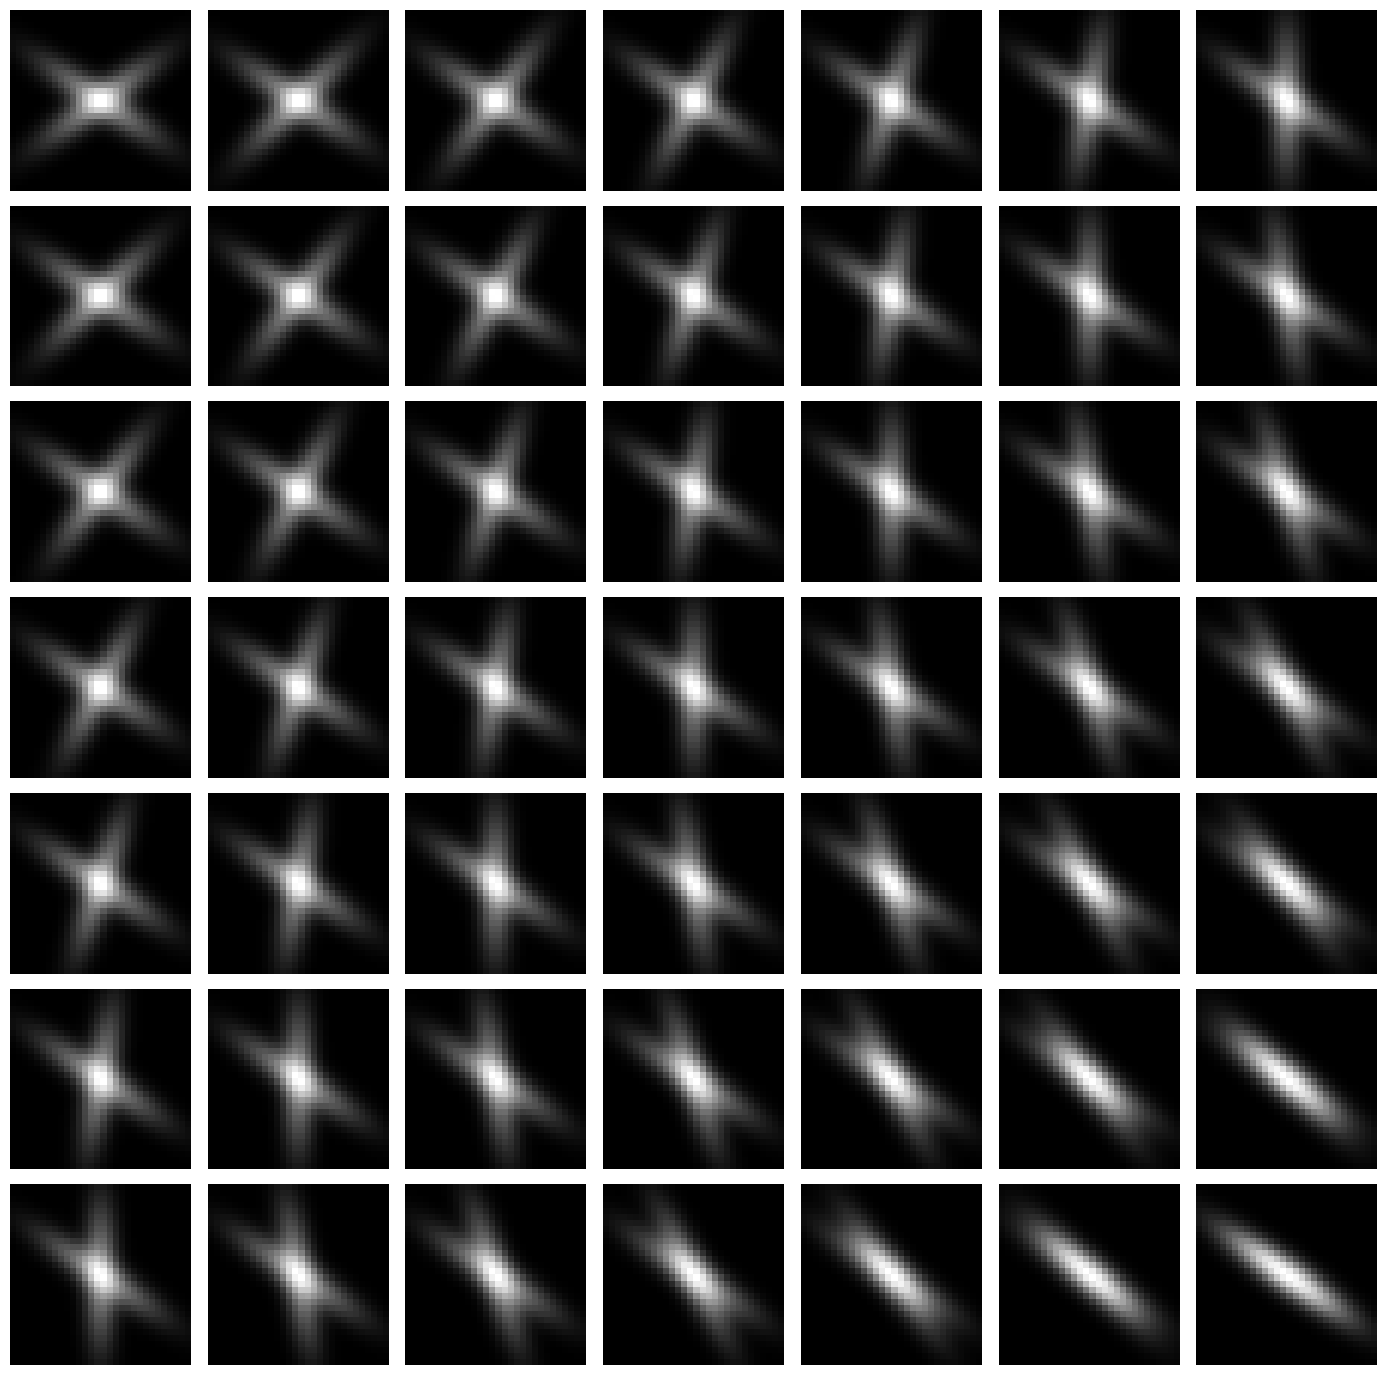
\includegraphics[width=\columnwidth]{img/full_displacements.png}}
    \caption{Representation of the synthetic data $P^\dag$: each separate square represents the displacement distribution within the voxel.}
    \label{fig:full_displacements}
    \end{figure}
    \begin{figure}[!t]
    \centerline{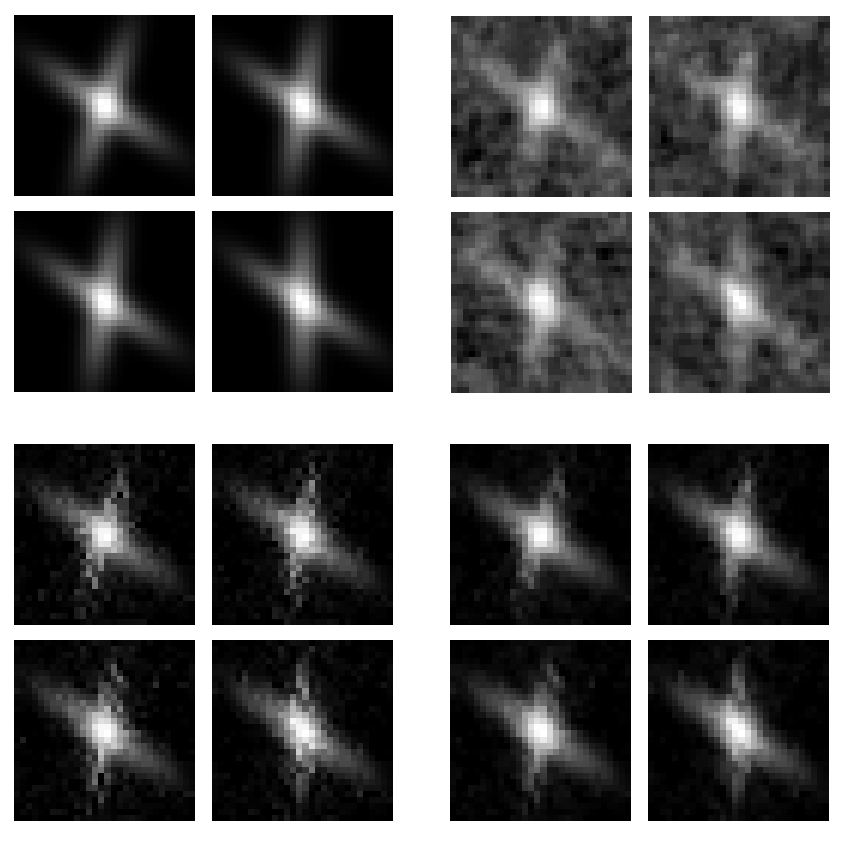
\includegraphics[width=\columnwidth]{img/reconstruction_details.png}}
    \caption{Detail of the reconstructions: we have selected a $2\times2$ area corresponding to $2 \le i,j \le 3$. \textbf{Top left}: original data, for comparison. \textbf{Top right}: unregularized reconstruction (as a result of $\mathcal{F}^*(\mathcal{U}^*(E))$, i..e. the Moore-Penrose pseudoinverse). \textbf{Bottom left}: regularized reconstruction, with $\alpha_1=\alpha_2=0.002$ and $\beta=0$ (no voxelwise regularization). \textbf{Bottom right}: regularized reconstruction, with $\alpha_1=\alpha_2=0.002$ and $\beta=0.03$ (full model regularization).}
    \label{fig:reconstruction_details}
\end{figure}
%
To provide a controlled and interpretable test case, we first simulate a synthetic dataset defined on a 4D domain: a two-dimensional spatial grid $\Omega \subset \mathbb{R}^2$ and a two-dimensional displacement domain $Y \subset \mathbb{R}^2$. This reduced setting allows for direct visualization of both the EAP structure and the effect of regularization across space and displacement.

Each voxel in $\Omega$ contains a mixture of two oriented Gaussians in $Y$, modeling a crossing fiber configuration. One component is fixed across all voxels, while the second rotates spatially to create a varying crossing pattern. This setup induces strong spatial correlation in the displacement structure, which the proposed $\mathrm{TV}_{\hat{W}_1}$ regularizer is designed to exploit. The synthetic data $P^\dag$ has a shape of $7\times7\times30\times30$.
To simulate q-space undersampling, we applied a binary mask to the displacement dimensions of the 4D Fourier-transformed signal \( \mathcal{F}(P^\dag) \), where $P^\dag$ is the ground truth EAP. The mask is shared across all spatial positions \( (i,j) \), and retains 20\% of the displacement frequency components, selected according to a variable-density Gaussian distribution centered at the origin of q-space. The observed data
\[
E = \mathcal{U}(\mathcal{F}(P^\dag)) + \eta,
\]
where $\mathcal{U\circ F}$ is the undersampled Fourier Transform as previously introduced, and \( \eta \) is entrywise i.i.d. Gaussian noise drawn from \( \mathcal{N}(0, \sigma^2) \), with $ \sigma = 0.01 \cdot \mathrm{max}_{i} \{ |E_i| \} $.

An illustration of this 4D structure is shown in Fig. \ref{fig:full_displacements}, where each square corresponds to a voxel containing the displacement distributions over $Y$. Reconstruction details are shown in Fig. \ref{fig:reconstruction_details}.

\subsection{Realistic Crossing Fibers}
\textit{Thom's work}\\
To move toward more realistic conditions, we also test our method on simulated data derived from ground truth diffusion profiles generated using standard diffusion modeling software. In this case, fiber crossings are modeled at sub-voxel scale using predefined orientations and volume fractions. Details of the data generation and acquisition model will be provided in the final version. As in the synthetic case, the data is subsampled and corrupted with noise, and we evaluate the quality of reconstruction using both visual inspection and quantitative metrics (e.g., angular error, RMSE, sparsity structure).

\subsection{Parameter tuning}
\begin{figure}[!t]
\centerline{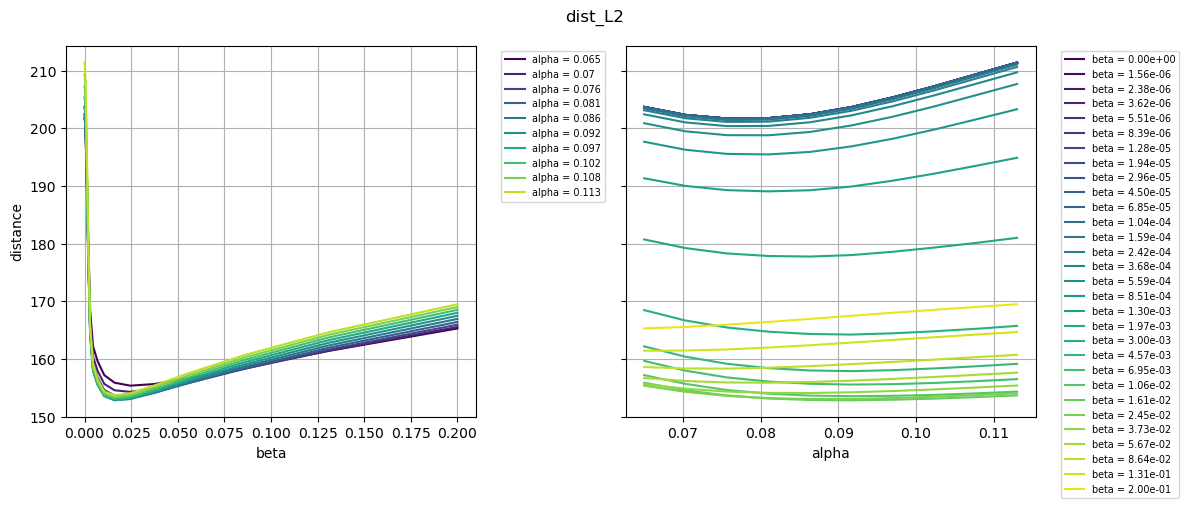
\includegraphics[width=\columnwidth]{img/parameter tuning.png}}
\caption{ }
\label{fig:}
\end{figure}

\section{Conclusion}
Conclusion

\appendix
\section*{Appendix}
\subsection{Notation}

\subsection{Solving the variational problem}

\section*{Useful literature (temporary section)}
\begin{itemize}
    \item \href{chrome-extension://efaidnbmnnnibpcajpcglclefindmkaj/https://arxiv.org/pdf/1707.09958}{(kq)-Compressed Sensing for dMRI with Joint Spatial-Angular Sparsity Prior}: overview of compressed sensing for DSI
    \item \href{https://drive.google.com/file/d/19IQJwwOZqE2nf86KQN4G5pCdBtBXqUcw/view?usp=sharing}{Leveraging EAP-Sparsity for Compressed Sensing of MS-HARDI in (k, q)-Space}: Use of TV-type regularization
    \item Thom's suggestions
    \href{https://link.springer.com/article/10.1007/s002340050020}{Reducing motion artefacts in diffusion-weighted MRI of the brain: efficacy of navigator echo correction and pulse triggering}\\
    \href{https://www.ejradiology.com/article/S0720-048X(02)00303-0/fulltext}{Basic principles of diffusion-weighted imaging
}
\end{itemize}

\section{Paper Roadmap}

\subsection{Title and Abstract}
\begin{itemize}
    \item Consider making title more specific about the application domain
    \item Abstract needs quantitative results
    \item Add 5-8 relevant keywords (diffusion MRI, optimal transport, total variation, compressed sensing, image reconstruction, etc)
\end{itemize}

\subsection{Introduction}
\begin{itemize}
    \item Add specific clinical applications (tractography, brain connectivity, disease diagnosis)
    \item Expand on acquisition time limitations, noise, undersampling artifacts
    \item Comprehensive literature review of existing methods:
    \begin{itemize}
        \item Classical methods (DTI, HARDI, Q-ball)
        \item Compressed sensing approaches for dMRI
        \item Total variation methods in medical imaging
        \item Optimal transport applications in imaging
    \end{itemize}
    \item Clear gap analysis showing limitations of current methods
    \item Specific, numbered contributions with novelty claims
    \item Brief outline of paper organization
\end{itemize}

\subsection{Background and Related Work}
\begin{itemize}
    \item Diffusion MRI physics: signal equation, b-values, q-space sampling
    \item Compressed sensing for dMRI: prior art, limitations
    \item Total variation regularization: classical TV, extensions to vector/tensor fields
    \item Optimal transport theory: Wasserstein distances, applications in imaging
    \item Joint (k,q)-space reconstruction: existing approaches and their limitations
\end{itemize}

\subsection{Notation and Mathematical Preliminaries}
\begin{itemize}
    \item Standardized notation table for all variables:
    \begin{itemize}
        \item Spatial domain $\Omega$, displacement domain $Y$
        \item EAP $P(x,r)$, signal $E(k,q)$
        \item Operators: Fourier transform $\mathcal{F}$, undersampling $U$
        \item Norms and metrics
    \end{itemize}
    \item Mathematical definitions of key concepts
\end{itemize}

\subsection{Methodology}
\begin{itemize}
    \item Complete variational model with all terms explained
    \item Algorithm development:
    \begin{itemize}
        \item Primal-dual algorithm details
        \item Convergence properties ?!?
        \item Computational complexity analysis
    \end{itemize}
    \item Implementation details:
    \begin{itemize}
        \item Discretization schemes
        \item Boundary conditions
        \item Parameter selection strategies
    \end{itemize}
    \item Relationship to existing methods
\end{itemize}

\subsection{Experimental Design and Validation}

\subsubsection{Synthetic Data Experiments}
\begin{itemize}
    \item Expand synthetic tests:
    \begin{itemize}
        \item 3D spatial + 3D displacement scenarios
        \item Various fiber configurations (single, crossing, kissing, fanning)
        \item Different noise levels and undersampling ratios
        \item Ground truth generation methodology
    \end{itemize}
\end{itemize}

\subsubsection{Semi-Realistic Data}
\begin{itemize}
    \item Simulation framework:
    \begin{itemize}
        \item Fiber phantoms with known ground truth
        \item Realistic acquisition parameters
        \item Comparison with analytical solutions where possible
    \end{itemize}
\end{itemize}

\subsubsection{Real Data Validation}
\begin{itemize}
    \item Dataset description:
    \begin{itemize}
        \item Human brain data (healthy subjects)
        \item Acquisition parameters (scanner, sequences, b-values)
        \item Data preprocessing pipeline
    \end{itemize}
    \item Clinical datasets:
    \begin{itemize}
        \item Pathological cases for clinical relevance (if available)
        \item Multi-site validation for robustness
    \end{itemize}
\end{itemize}

\subsection{Experimental Results}

\subsubsection{Quantitative Metrics}
\begin{itemize}
    \item Image quality metrics:
    \begin{itemize}
        \item RMSE, PSNR, SSIM for EAP reconstruction
        \item Angular error for fiber orientations
        \item FA, MD accuracy in ROIs
    \end{itemize}
    \item Fiber-specific metrics:
    \begin{itemize}
        \item Tractography accuracy (if applicable)
        \item Crossing angle estimation error
        \item Volume fraction accuracy
    \end{itemize}
\end{itemize}

\subsubsection{Comparison Studies}
\begin{itemize}
    \item Baseline methods:
    \begin{itemize}
        \item Standard least squares reconstruction
        \item Classical TV regularization
        \item State-of-the-art dMRI reconstruction (HARDI, DSI, etc.)
        \item Recent compressed sensing methods for dMRI
    \end{itemize}
    \item Ablation studies:
    \begin{itemize}
        \item Effect of each regularization term
        \item Parameter sensitivity analysis
        \item Computational time comparisons
    \end{itemize}
\end{itemize}

\subsubsection{Visual Results}
\begin{itemize}
    \item Reconstruction quality: side-by-side comparisons with ground truth
    \item EAP visualizations: 3D displacement probability surfaces
    \item ROI analysis: detailed analysis in regions of interest
    \item Error maps: spatial distribution of reconstruction errors
\end{itemize}

\subsection{Computational Aspects}
\begin{itemize}
    \item Algorithm efficiency:
    \begin{itemize}
        \item Convergence rates
        \item Memory requirements
        \item Scalability analysis
    \end{itemize}
    \item Implementation details:
    \begin{itemize}
        \item Programming language, libraries
        \item Hardware specifications
        \item Runtime comparisons
    \end{itemize}
\end{itemize}

\subsection{Discussion}
\begin{itemize}
    \item Key findings: interpretation of results
    \item Clinical implications: relevance to medical applications
    \item Method advantages: when and why the method works
    \item Limitations:
    \begin{itemize}
        \item Computational requirements
        \item Parameter tuning requirements
        \item Applicability constraints
    \end{itemize}
    \item Future directions:
    \begin{itemize}
        \item Extension to other MRI modalities
        \item Real-time reconstruction possibilities
        \item Integration with clinical workflows
    \end{itemize}
\end{itemize}

\subsection{Conclusion}
\begin{itemize}
    \item Summary of contributions: concise restatement
    \item Clinical impact: potential benefits for medical practice
    \item Technical advances: novel algorithmic contributions
\end{itemize}

\subsection{Appendices}

\subsubsection{Mathematical Details}
\begin{itemize}
    \item Optimization derivations: move detailed math here
    \item Primal-dual algorithm: complete algorithmic details
    \item Convergence proofs (if available)
    \item Computational complexity: detailed analysis
\end{itemize}

\subsubsection{Implementation Details}
\begin{itemize}
    \item Parameter settings: complete parameter tables
    \item Preprocessing steps: detailed data preparation
    \item Reproducibility information: code availability, exact parameters
\end{itemize}

\subsection{Supplementary Material}
\begin{itemize}
    \item Additional results: extended comparisons, more datasets
    \item Video materials: 3D visualizations of EAP reconstructions
    \item Code repository: link to implementation
\end{itemize}

\subsection{Required Figures}
\begin{enumerate}
    \item Method overview: flowchart of the reconstruction pipeline
    \item Synthetic data setup: visualization of test configurations
    \item Quantitative comparisons: performance metrics across methods
    \item Visual comparisons: side-by-side reconstruction results
    \item Parameter sensitivity: effects of regularization parameters
    \item Real data results: clinical dataset reconstructions
    \item ROI analysis: detailed regional analysis
    \item Convergence plots: algorithm convergence behavior
\end{enumerate}

\subsection{Required Tables}
\begin{enumerate}
    \item Notation table: all mathematical symbols
    \item Dataset specifications: acquisition parameters
    \item Quantitative results: numerical comparison with baselines
    \item Computational performance: runtime and memory usage
    \item Parameter settings: optimal parameters for different scenarios
\end{enumerate}

\subsection{Quality Assurance Checklist}

\subsubsection{Technical Requirements}
\begin{itemize}
    \item Mathematical rigor: all equations properly derived and cited
    \item Reproducibility: sufficient detail for reproduction
    \item Statistical significance: proper statistical testing of results
    \item Validation: comprehensive comparison with state-of-the-art
\end{itemize}

\subsubsection{IEEE TMI Specific Requirements}
\begin{itemize}
    \item Clinical relevance: clear medical application
    \item Innovation: novel technical contribution
    \item Comprehensive evaluation: multiple datasets, metrics, comparisons
    \item High-quality figures: publication-ready visualizations
    \item Proper citations: complete literature review
\end{itemize}

\subsubsection{Writing Quality}
\begin{itemize}
    \item Clarity: accessible to medical imaging community
    \item Flow: logical progression of ideas
    \item Conciseness: within page limits
\end{itemize}

\subsection{Critical Success Factors}
\begin{enumerate}
    \item Strong quantitative results: demonstrate clear improvement over baselines
    \item Clinical validation: show relevance to real medical scenarios
    \item Comprehensive comparison: fair evaluation against state-of-the-art
    \item Reproducible research: provide sufficient implementation details
    \item Clear innovation: articulate novel contributions effectively
\end{enumerate}


\appendices

\section*{Appendix}

\section*{Acknowledgment}
Acknowledgment


\begin{thebibliography}{00}

\bibitem{LeveragingEAP}
Sun J, Sakhaee E, Entezari A, Vemuri BC. Leveraging EAP-Sparsity for Compressed Sensing of MS-HARDI in (k, q)-Space. Inf Process Med Imaging. 2015;24:375-86. doi: 10.1007/978-3-319-19992-4\_29. PMID: 26221688; PMCID: PMC4807403.

\bibitem{VogtLellmann1}
Vogt, T., Lellmann, J. (2017). An Optimal Transport-Based Restoration Method for Q-Ball Imaging. In: Lauze, F., Dong, Y., Dahl, A. (eds) Scale Space and Variational Methods in Computer Vision. SSVM 2017. Lecture Notes in Computer Science(), vol 10302. Springer, Cham. https://doi.org/10.1007/978-3-319-58771-4\_22

\bibitem{TVW_Theory}
TVW1 Theory (\textcolor{red}{to be uploaded soon})

\bibitem{review_kq_compressed_sensing} 
Schwab, E., Vidal, R., Charon, N. (2017). (k,q)-compressed sensing for dMRI with joint spatial-angular sparsity prior. In arXiv [cs.CV]. https://doi.org/10.48550/ARXIV.1707.09958

\end{thebibliography}

\end{document}
